
\section{Mécanique des failles}
\label{sec:failles}






La mécanique des failles est le domaine de la géophysique étudiant les mécanismes de déformations des roches et des failles sismiques, au travers d'échelles de temps et d'espace très diverses. Dans le cadre de notre étude d'une faille en laboratoire nous cherchons à caractériser des mouvements de glissement rapide à l'interface, qui s'apparentent à des séismes, un des objets d'étude de la mécanique des failles. Nous présentons dans cette section les principes de base de l'étude des mouvements lithosphériques, de la tectonique des plaques, et de la mesure et la caractérisation des séismes.


\begin{figure}[hbt]
\centering

\includegraphics[scale=1]{../Figures_chap_article/failles.pdf}
\caption[Types de failles]{Les trois grands types de failles. La faille normale (\textbf{a}) apparaît dans les systèmes en extension. La faille inverse (\textbf{b}) apparaît dans les systèmes en compression comme les zones de subduction. La faille transformante (\textbf{c}) apparaît dans les zones de coulissement entre des plaques tectoniques.}
\label{fig:typesdefailles2}
\end{figure}

\subsection{Qu'est-ce qu'une faille ?}

En géologie, une \textit{faille} est un plan ou une zone de rupture entre deux blocs rocheux qui sont en déplacement relatif. Les failles peuvent être de grandes dimensions, comme les failles tectoniques, ou millimétriques. Ces failles peuvent former des plans de ruptures très nets et très actifs, comme la faille de San Andreas à l'ouest des États-Unis\,\cite{scholz_evidence_2000}, ou de grandes zones de rupture contenant de multiples failles individuellement peu actives comme le rift est-africain\,\cite{chorowicz_east_2005}.




\subsubsection{Origine des failles}


La croûte terrestre, ou \textit{lithosphère}, est composée de plaques en mouvement relatif. Ces plaques, dites \textit{plaques tectoniques}, d'une épaisseur d'environ \SI{100}{\kilo\meter}\,\cite{pollack_regional_1977}, sont composées de roches basaltiques et granitiques solides et rigides, et reposent sur l'\textit{asthénosphère}, ou manteau terrestre, composé pour sa part de péridotites dans un état solide, mais ductile (Fig.\,\ref{fig:tecto}a). Le manteau, d'une épaisseur de l'ordre de \SI{3000}{\kilo\meter}, a une viscosité de l'ordre de $10^{18}$ à $10^{22}$\,Pa.s  contre $10^{25}$ pour la lithosphère\,\cite{cathles_viscosity_2015}, et peut ainsi, sous l'influence des gradients de température au sein de la Terre, adopter un mouvement de convection (Fig.\,\ref{fig:tecto}b). Ces mouvements forment des rouleaux, qui entraînent avec eux les plaques tectoniques à des vitesses allant jusqu'à \SI{10}{\centi\meter} par an.

De nombreux phénomènes géologiques ont lieu à l'interface entre les plaques tectoniques. Les zones d’accrétion, situées à l'interface entre deux plaques en éloignement, sont le siège d'un volcanisme à l'origine par exemple de la dorsale Atlantique qui émerge en Islande. Dans les zones de collision entre deux plaques, les mouvements tectoniques sont responsables de la subduction de la lithosphère océanique, engendrant du volcanisme d'arc, partiellement à l'origine de la lithosphère continentale\,\cite{stern_subduction_2002,Hawkesworth_generation_2010}. Des mouvements de coulissement entre les plaques tectoniques peuvent également se produire, comme c'est le cas le long de la faille de San Andreas\,\cite{anderson_san_1971, okubo_fractal_1987,zoback_new_1987, powell_evolution_1992, linde_slow_1996, tan_connecting_2020}. Les failles ont une morphologie sculptée par le temps et les contraintes qu'elles subissent.

\begin{figure}[hbt]
\centering
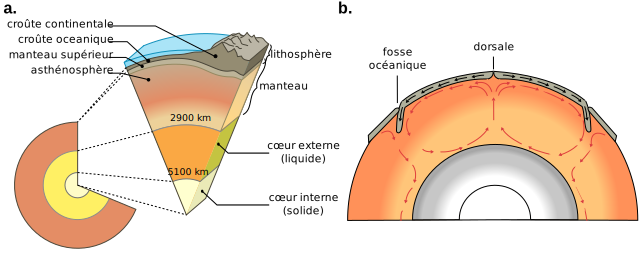
\includegraphics[scale=1]{../Figures_chap_intro/coupeterre.pdf}
\caption[Structure interne de la Terre]{Schéma de la structure interne de la Terre et du mécanisme par lequel les mouvements de convection du manteau sont à l'origine de la tectonique des plaques.}
\label{fig:tecto}
\end{figure}


\subsubsection{Anatomie d'une faille}



Une faille est un système géophysique complexe, centré sur un plan de faille, et composé de multiples couches de roches structurellement et chimiquement différentes. Lorsque deux blocs de roches en contact sont soumis à un déplacement relatif, ils subissent des contraintes et déformations menant à la fragilisation et à l'usure des roches. Il est ainsi possible d'observer de part et d'autre du plan de faille une succession de couches géologiques aux propriétés variées.

À grande distance du plan de faille, la roche mère forme un bloc solide, accumulant de l'énergie élastique au travers des déformations qu'elle subit. En s'approchant de la faille et en entrant dans la zone d'endommagement, celle-ci devient une \textit{cataclastite}, une roche de faille fracturée, broyée et stratifiée par le déplacement relatif des deux blocs en contact (Fig.\,\ref{fig:faillereelle}). Au centre de la zone de faille se trouve la zone cœur, composée de brèche de faille et de gouge, une roche granulaire non cohésive\,\cite{woodcock_classification_2008}. Au delà des différences de granulométrie, la différence de porosité entre ces couches introduit également des différences chimiques et métamorphiques. Enfin les failles sismiques ont une extension spatiale en profondeur, des séismes pouvant se produire jusqu'à 600 kilomètres sous la surface\,\cite{frohlich_nature_1989}. Chaque système de faille a sa morphologie propre.


\begin{figure}[h!]
\centering
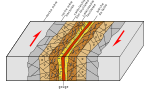
\includegraphics[scale=1]{../Figures_chap_article/realfault.pdf}
\caption[Anatomie d'une faille]{Anatomie schématique d'une faille sismique réelle. La faille est composée de multiples couches de roches, plus ou moins cohésives et fracturées. Les couches de brèche et de gouge sont des milieux granulaires au cœur de la faille (adapté de\,\cite{treffeisen_fault_2021}).}
\label{fig:faillereelle}
\end{figure}



\subsection{Étude des séismes}


Lorsque deux plaques tectoniques sont en contact, elles sont soumises à des forces de frottement solide. Les zones la plupart du temps bloquées en surface sont toujours soumises aux contraintes appliquées par les déplacements de l'asthénosphère, et accumulent de l'énergie élastique au travers de leurs déformations. Lorsqu'elles se débloquent, un évènement de glissement rapide a lieu. Cet évènement, relâchant l'énergie élastique accumulée, dure généralement au plus quelques secondes, et émet des ondes de déformations qui se propagent dans les roches alentour, parfois jusqu'à la surface. C'est ce mécanisme que l'on nomme \textit{séisme}.

%Les roches en contacts sont plus ou moins visqueuses selon les conditions de température et de pression dans lesquelles elles évoluent\,\cite{mccaffrey_slow_2008}, 



\subsubsection{Le stick-slip comme description du cycle sismique}

Les séismes sont la manifestation d'un mouvement de stick-slip. Cette observation, publiée en 1966 par W.\,F.\,Brace et J.\,D.\,Byerlee\,\cite{brace_stick-slip_1966}, s'appuyant alors sur les études menées en laboratoire sur des roches naturelles\,\cite{jaeger_frictional_1959,uffen_stress_1963,griggs_observations_1960}, est un fondement de l'étude moderne de la sismicité, remplaçant la théorie du rebond élastique de Reid\,\cite{reid_mechanics_1910}. Le mouvement de stick-slip est en effet caractéristique des dynamiques régies par les frottements solides (Sec.\,\ref{sec:ss1}).

Dans les mouvements géologiques ce mouvement de stick-slip ne se caractérise cependant pas par sa régularité, puisqu'il est très difficile de prédire les séismes\,\cite{rikitake_earthquake_1968, mogi_earthquake_1985, geller_earthquake_1997, kanamori_earthquake_2003}. La prédiction et prévention de ceux-ci est pourtant un enjeu majeur, et la compréhension des mécanismes microscopiques sous-jacents au frottement solide en est une clé. L'étude de ces mécanismes a mené à de nombreux modèles empiriques (Sec.\,\ref{sec:rateandstate}) appuyés par des observations de terrain permettant de décrire le comportement des failles et de rendre compte de ce phénomène de stick-slip à l'échelle des temps géologique.


\subsubsection{Magnitude et moment sismique}

Un séisme est la manifestation d'un glissement le long d'une interface frictionnelle. Il s'accompagne d'une dissipation d'énergie (Éq.\,\ref{eq:dissip}) et de l'émission et la propagation d'ondes dans les roches. La mesure de ces phénomènes permet de définir des grandeurs utiles à la caractérisation, au catalogage et à l'étude statistique des séismes. Nous définissons ici plusieurs de ces observables.


\myparagraph{Le déplacement moyen}

\begin{figure}[htb]
\centering
\includegraphics[width=.8\textwidth]{../Figures_chap_intro/fence.jpg}
\caption[Observation directe du glissement dû à un séisme]{Photographie des effets du tremblement de terre de 1906 à San Francisco, causé par la rupture d'une portion de la faille de San Andreas. La faille a glissé d'environ \SI{2.5}{\meter} le long d'un plan de fissure particulièrement bien défini\,\cite{reid_mechanics_1910}.}
\label{fig:fence}
\end{figure}

Le déplacement moyen est la moyenne de la distance glissée le long de la faille ou portion de faille rompue lors d'un séisme (Fig.\,\ref{fig:fence}). Son évaluation peut être effectuée par mesure directe des glissements sur le terrain, cependant dès lors que le mouvement est faible, ou que la zone de faille est étendue, elle perd en précision. Des techniques d'imagerie satellite ou de mesure par balises GPS permettent de raffiner ces mesures à une précision de l'ordre du centimètre, et de déterminer le champ des déformations dans toute la lithosphère\,\cite{michel_measuring_1999,segall_gps_1997,pagani_quantification_2021}. La mesure des déplacements en surface ne suffit cependant pas à caractériser un séisme, puisque certains mouvements profonds ne s'accompagnent pas d'un glissement en surface. Pour les caractériser des grandeurs liées à l'énergie qu'ils relâchent sont utilisées.


\myparagraph{Les magnitudes}

La \textit{magnitude} d'un séisme est une grandeur sans unité évaluant l'énergie libérée par ce séisme sur une échelle logarithmique. Sa définition a évolué au cours du temps, en fonction de la grandeur mécanique utilisée pour la mesurer. Historiquement la première définition est celle de Richter en 1935 de la magnitude locale $M_L$\,\cite{richter_instrumental_1935}. Elle est basée sur les mesures des ondes sismiques par des sismographes, appareils combinant des accéléromètres et vélocimètres, et est définie comme

\begin{equation}
M_L=\log(D)-\log(D_0)+c\times\log(\Delta)
\end{equation}

Dans cette équation, $D$ désigne l'amplitude maximale mesurée sur le sismogramme utilisé pour la mesure, $\Delta$ la distance à l'épicentre, $c$ une constante d'étalonnage, et $D_0$ une amplitude de référence déterminant ce que l'on considère comme la valeur de $D$ pour un séisme de magnitude $M_L=0$ perçu à \SI{100}{\kilo\meter}. Cette définition est aujourd'hui limitée à des études locales, car elle dépend de paramètres empiriques locaux, étalonnés par zone de faille. Cette limitation à mené à la définition des \textit{magnitudes d'ondes} basées chacune sur la mesure d'un type d'onde spécifique. Les deux magnitudes d'ondes sont celle des ondes de surface $M_S$ et celle des ondes de volume (\textit{body waves}) $m_b$ toutes deux introduites par Gutenberg et Richter en 1936 et 1956\,\cite{gutenberg_magnitude_1936,gutenberg_earthquake_1956}. Toujours en usage aujourd'hui, elles demeurent empiriques et basées sur des étalonnages, et subissent un phénomène de saturation lorsque $M_S$ ou $m_b>9$\,\cite{kanamori_energy_1977, howell_saturation_1981}.

La magnitude la plus couramment utilisée aujourd'hui est la \textit{magnitude de moment} $M_w$ introduite par Hanks et Kanamori en 1979\,\cite{hanks_moment_1979}, liée directement à l'énergie libérée par le séisme et au moment sismique. Elle est particulièrement utilisée pour les séismes de grande magnitude ($M>4$), tandis que les magnitudes d'ondes sont privilégiées pour les faibles magnitudes.

\myparagraph{Le moment sismique}

le \textit{moment sismique} $M_0$ est une mesure de l'énergie libérée par un séisme par l'évaluation du travail des forces responsables du glissement. À longue distance un séisme peut en effet être vu comme le résultat de l'application d'un double couple de forces\,\cite{kagan_3-D_1991} résultant en une déformation élastique des roches. Le moment s'exprime alors comme

\begin{equation}
M_0=\frac{E}{2(1+\nu)}\times A\times d
\end{equation}

Dans cette équation $G_s=E/2(1+\nu)$ est le module de cisaillement, $A$ est la surface macroscopique du plan de fracture rompue durant l'évènement, et $d$ est le déplacement moyen à l'interface. La magnitude de moment est alors définie comme

\begin{equation}
M_w=\frac{2}{3}\log_{10}(M_0)-6.07
\label{eq:magnitude}
\end{equation}

Une augmentation d'un point de magnitude correspond à une multiplication par 30 du moment sismique. La magnitude est ainsi définie sur une échelle à valeurs dans $\mathbb{R}$ nommée \textit{échelle de Richter}\,\cite{kanamori_quantification_1978}. L'échelle est théoriquement illimitée, cependant le séisme le plus fort enregistré est le séisme de 1960 à Valdivia au Chili, avec une magnitude $M_w=9.5$\,\cite{ruiz_historical_2018}. Les tremblements de terre d'une telle magnitude n'ont lieu qu'une à trois fois par siècle, et relâchent une quantité suffisante d'énergie pour altérer l'axe de rotation de la Terre et changer la longueur du jour de quelques microsecondes\,\cite{chao_changes_1987}. Bien que l'échelle n'ait théoriquement pas non plus de minimum, les séismes de magnitude inférieure à 1 sont très difficilement détectables et se produisent en continu sur Terre. Ils peuvent même être dus aux activités humaines, un séisme de magnitude 0 relâchant une quantité d'énergie équivalente à celle libérée par la
chute d'un objet d'une tonne d'une hauteur de \SI{5}{\meter}.
%\href{https://youtu.be/e3uk7jU3RHo}{\textcolor{black}{chute d'un objet d'une tonne d'une hauteur de \SI{5}{\meter}}.}

Dans le but de décrire et prévenir les risques sismiques, le moment sismique et la magnitude font l'objet d'études statistiques et de modèle empiriques, comme la loi de Gutenberg-Richter.


\subsubsection{Loi de Gutenberg Richter}

\label{sec:gutricht}

\begin{figure}[htb]
\centering
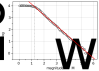
\includegraphics[scale=1]{../Figures_chap_intro/grlaw.pdf}
\caption[Loi de Gutenberg-Richter]{Distribution fréquence-magnitude cumulée des évènements sismiques dans la région de Abruzzi en Italie, entre avril 2007 et avril 2010 (adapté de\,\cite{de_santis_gutenberg-richter_2011}). Un séisme de magnitude $M_w=6.3$ a eu lieu dans la zone surveillée le 6 avril 2009. Un ajustement de la portion linéaire de la distribution (ligne rouge) permet une estimation globale des paramètres de la loi de Gutenberg-Richter ($b=0.89\pm0.03$). La ligne verticale en pointillés représente une estimation de la magnitude minimale à partir de laquelle les sismographes perdent leur sensibilité.}
\label{fig:grlaw}
\end{figure}

La loi de Gutenberg-Richter est une loi empirique décrivant la distribution de magnitude des séismes dans un réseau de failles donné\,\cite{gutenberg_frequency_1944}. Cette loi exprime un lien entre la magnitude $M$ et le nombre total de séismes d'une magnitude inférieure à $M$ ou \textit{distribution fréquence-magnitude cumulée} noté $N_{>M}$. La loi de Gutenberg-Richter prédit qu'il existe des constantes $a$ et $b$ telles que
\begin{equation}
\log_{10}N_{>M}=a-bM
\label{eq:grlaw}
\end{equation}


La loi de Gutenberg-Richter, bien qu'empirique, dispose d'un bon accord avec les données des relevés sismiques (Fig.\,\ref{fig:grlaw}). Les paramètres de la loi sont cependant variables d'un système de failles à un autre, et sont mesurés par région sismique. L'accord aux données de terrain n'est valable qu'à partir d'une magnitude minimale $M^-$ car les évènements de magnitude inférieure ne sont pas détectés par les sismographes.

D'autres évènements de glissement peuvent échapper aux sismographes, comme les séismes lents (\textit{slow earthquakes})\,\cite{beroza_searching_1990}.
\vspace{1cm}
\pagebreak

\subsection{Mouvement asismique}

Le mouvement asismique est défini comme le glissement d'une portion de faille ne durant non pas quelques secondes comme un séisme mais des temps plus grands, allant de l'ordre de la minute à plusieurs années. Certaines failles sont même dites \textit{découplées}, c'est à dire en glissement permanent. Ces glissements ont été mesurés comme ayant des magnitudes allant jusqu'à $M_w=7$\,\cite{liu_recurrent_2015}. Le rôle de ce glissement lent dans le cycle sismique, et en particulier son influence dans le déclenchement de séismes de grande magnitude, ou au contraire dans le relâchement des contraintes, est un sujet de recherche actif et reste encore méconnu\,\cite{harris_large_2017, radiguet_triggering_2016,burgmann_geophysics_2018, leeman_frictional_2018,tan_connecting_2020}.


La compréhension des mécanismes entraînant le glissement lent de portions de failles ainsi que l'influence de ce glissement partiel d'une faille ou d'un système de failles sur ses portions bloquées sont deux motivations de notre étude. En particulier les expériences présentées dans le Chapitre\,\ref{sec:chaparticle} exposent un mécanisme par lequel ce glissement lent d'une portion d'une interface frictionnelle peut mener à une déstabilisation précoce, mais donc de magnitude moindre, du reste de l'interface.







